\documentclass[11pt]{article}
\usepackage{graphicx,listings}
\graphicspath{ {./images/} }
\title{\textbf{IoT 2023 Challenge 3}}
\author{
  Pasquale Castiglione\\
	\texttt{10657816}
  \and
  Lorenzo Campana\\
  \texttt{10605775}
}
\date{}
\begin{document}
\maketitle

\section{Introduction}
The goal of this challenge was to implement a routing algorithm in order to send a packet from Mote1 to Mote2.
\begin{figure}[h]
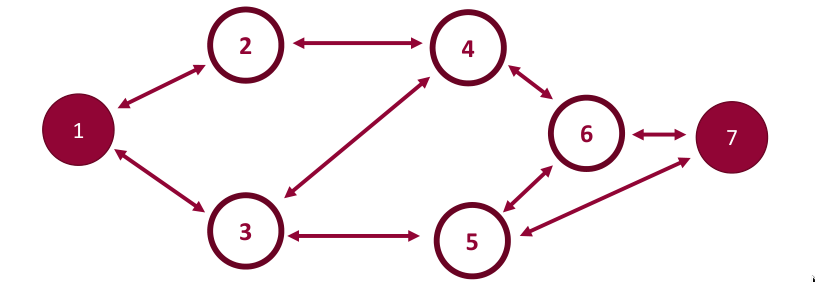
\includegraphics[width=\textwidth]{topology.png}
\caption{Network Topology}
\end{figure}
\section{Code}
\subsection{RadioRoute.h}
In the header file the data structures for the messages and for the routing table were defined.
\begin{lstlisting}[language=C]
typedef nx_struct radio_route_msg {
	nx_uint16_t type;
	nx_uint16_t sender;
	nx_uint16_t destination; // node_requested
	nx_uint16_t value; // cost
} radio_route_msg_t;
\end{lstlisting}

\begin{lstlisting}[language=C]
typedef struct route_entry_t {
	uint16_t next_hop;
  	uint16_t cost;
} route_entry_t;
\end{lstlisting}

\subsection{RadioRouteC.nc}
Two variables: \texttt{waiting\_packet} and \texttt{waiting\_address} were defined in order to store the message and the destination address to send when the routing table was empty.
At the beginning, right after the boot, the radio module was activated and a five seconds timer was started for the Mote 1.
\subsubsection{Send}
Before the sending of a message, the variabele \texttt{locked} is checked in order to check if the radio module is in use or not.
If the radio is free, 
\subsubsection{Receive}
Three types of message can be received:
\begin{itemize}
	\item{\textbf{Data Message}}
	\item{\textbf{Route Request}}
	\item{\textbf{Route Reply}}
\end{itemize}
\section{Results}
\end{document}
